%%% Local Variables:
%%% mode: latex
%%% TeX-master: "report"
%%% End:

% Section V: Results

The first result shown in figure~\ref{fig:result1} compares BER versus $E_b/N_0$ for small MIMO arrays and a stationary receiver. It can be seen that the uncoded $1\times1$ system performs the worst, followed by the diversity two $1\times2$ MRC system and the $2\times1$ Alamouti coded system, and then the diversity four $2\times2$ Alamouti coded system. This is in line with expected results discussed in the STBC section. Additionally, both QAM results are very close for each system, with the QPSK result being better for the uncoded system and worse for the other three coded systems. This suggests that ST coding is better at coding symbol angles rather than magnitudes.

The second result shown in figure~\ref{fig:result2} shows the results for $N_T=4$. The QAM results are again grouped together for each code, and so are the PSK results. It can be seen that the $C(4,3,4)$ and $C(4,4,4)$ codes are very close in performance for small $E_b/N_0$, so the QOSTBC code has a performance advantage in those cases with its greater spectral efficiency. Around 8~dB, is when the OSTBC starts outperforming the QOSTBC. However, the $C(4,2,4)$ code vastly performs the other two codes, since not only is it orthogonal, but it also has linear decoding. It performs about 3~dB better than the next best code for all modulation methods. This large gap in performance makes up for its reduced spectral efficiency.

Figure~\ref{fig:result3} compares the performance for various $N_T$ and $N_R=2$. There is a large gap between $N_T=1$ and $N_T=2$ and a even larger one between $N_T=2$ and $N_T=4$. The gap between $N_T=4$ and $N_T=8$ is much smaller in comparison and would likely need much larger constellation sizes and greater $E_b/N_0$ to distinguish between them clearly.

Figures~\ref{fig:result4a} through~\ref{fig:result5} show the extension of the previous results to moving receivers. For clarity of display, only the results for QPSK modulation are shown. The speeds are in m/s. It can be see that for the case of flat quasi-static Rayleigh fading, increasing the speed results in better performance, particularly for large $N_T$. This is due to the MRC used at the decoder favoring paths that shown greater gain under the fading. For a fast fading channel, this effect would likely not occur and worse performance would be expected.

\begin{figure}[p]
  \centering
  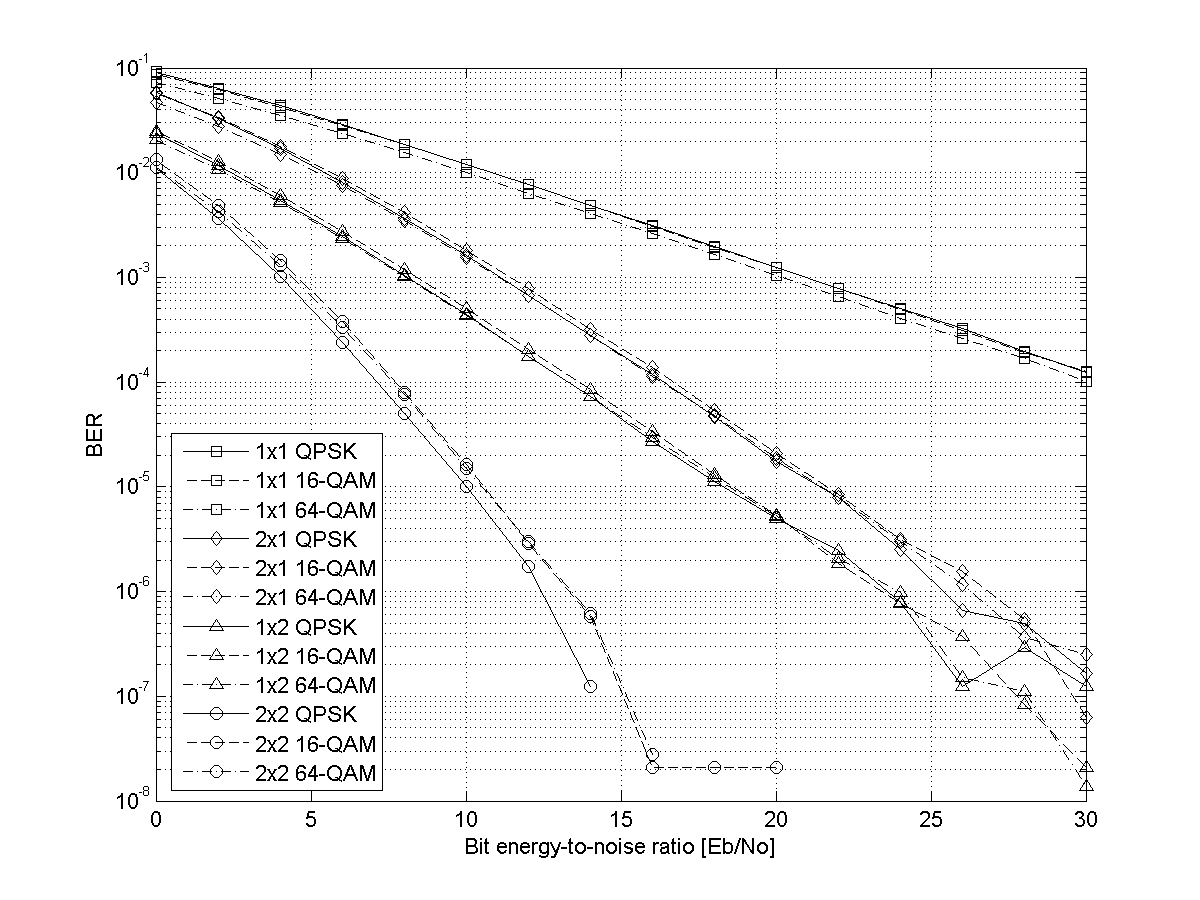
\includegraphics[width=0.8\textwidth]{images/result1.png}
  \caption{Comparison of BER versus $E_b/N_0$ for small MIMO and stationary receiver.}
  \label{fig:result1}
\end{figure}

\begin{figure}[p]
  \centering
  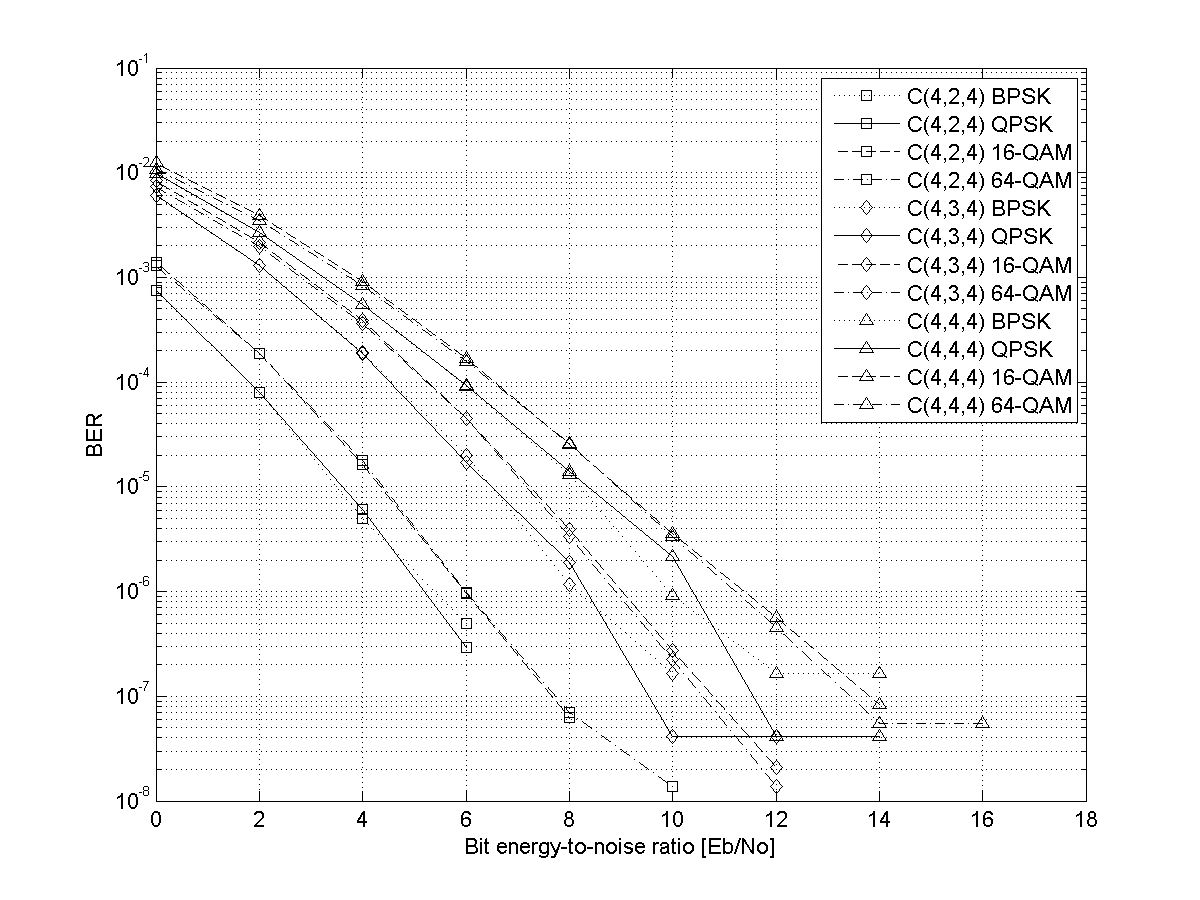
\includegraphics[width=0.8\textwidth]{images/result2.png}
  \caption{Comparison of BER versus $E_b/N_0$ for $N_T=4$ and stationary receiver.}
  \label{fig:result2}
\end{figure}

\begin{figure}[p]
  \centering
  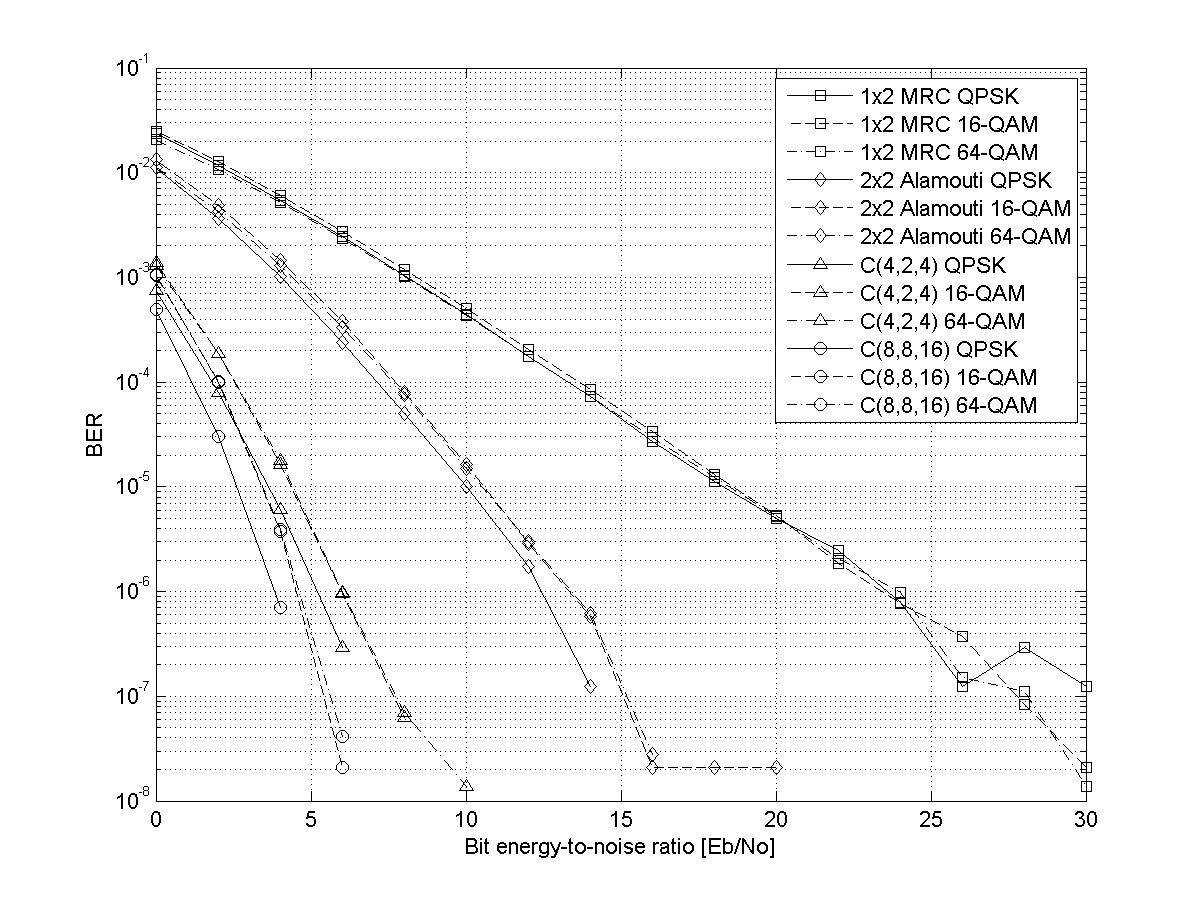
\includegraphics[width=0.8\textwidth]{images/result3.png}
  \caption{Comparison of BER versus $E_b/N_0$ for various $N_T$ and stationary receiver.}
  \label{fig:result3}
\end{figure}

\begin{figure}[p]
  \centering
  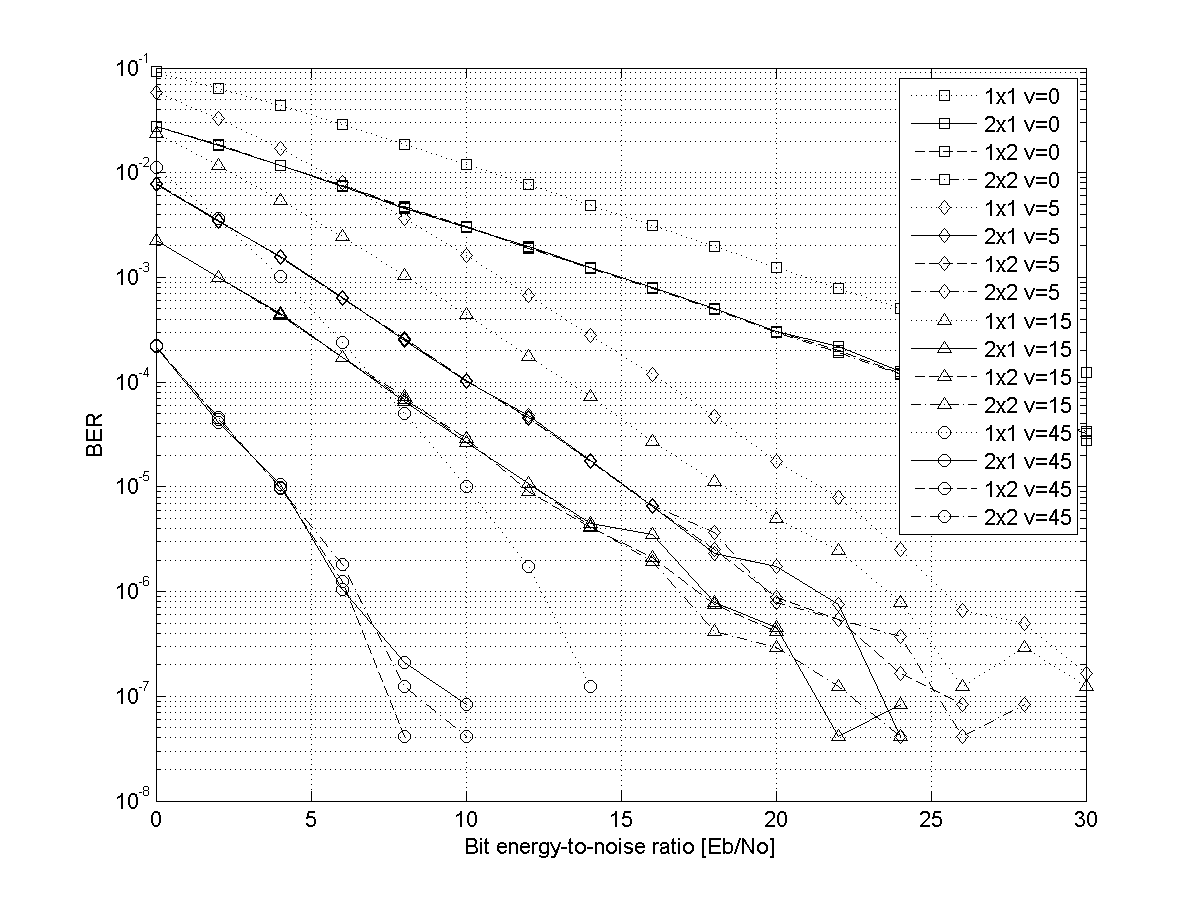
\includegraphics[width=0.8\textwidth]{images/result4a.png}
  \caption{Comparison of BER versus $E_b/N_0$ for QPSK, small MIMO, and moving receiver.}
  \label{fig:result4a}
\end{figure}

\begin{figure}[p]
  \centering
  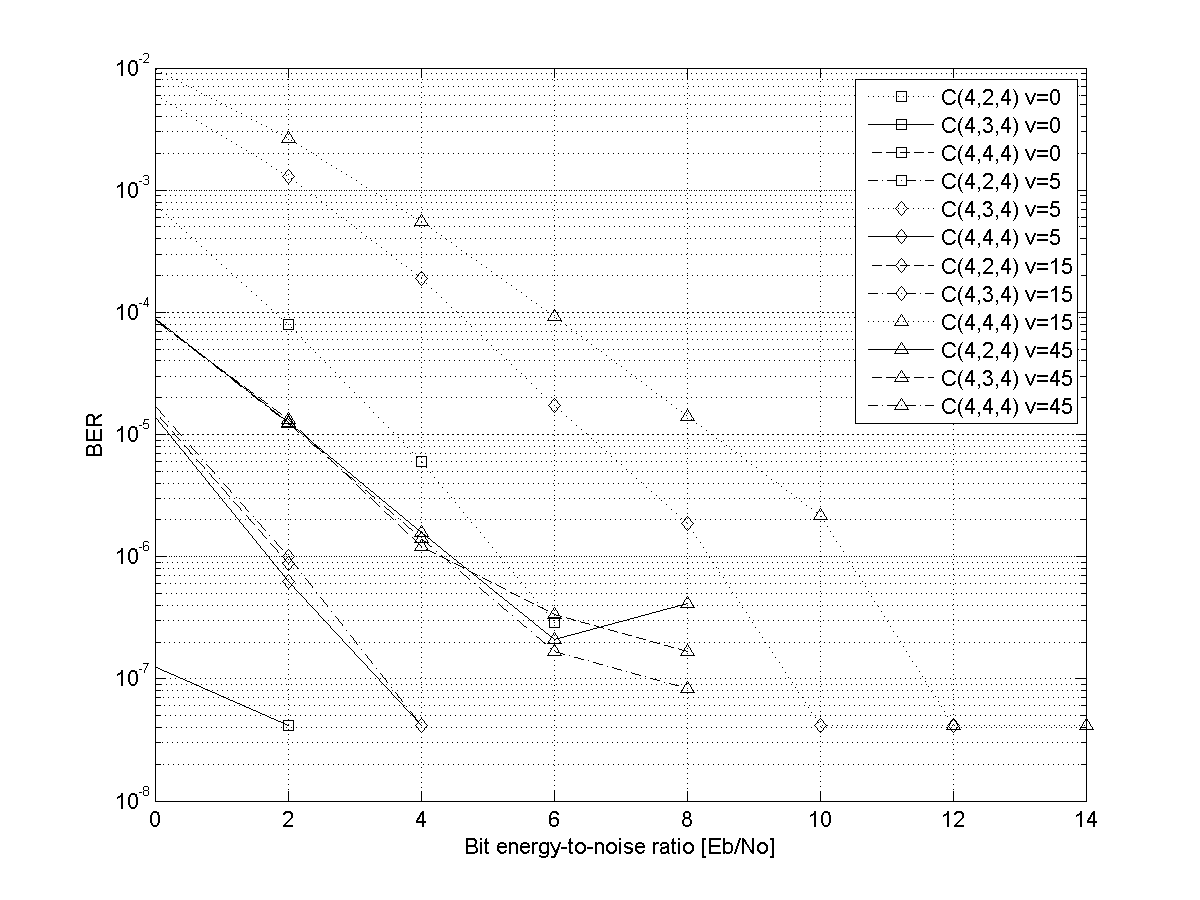
\includegraphics[width=0.8\textwidth]{images/result4b.png}
  \caption{Comparison of BER versus $E_b/N_0$ for QPSK, $N_T=4$, and moving receiver.}
  \label{fig:result4b}
\end{figure}

\begin{figure}[p]
  \centering
  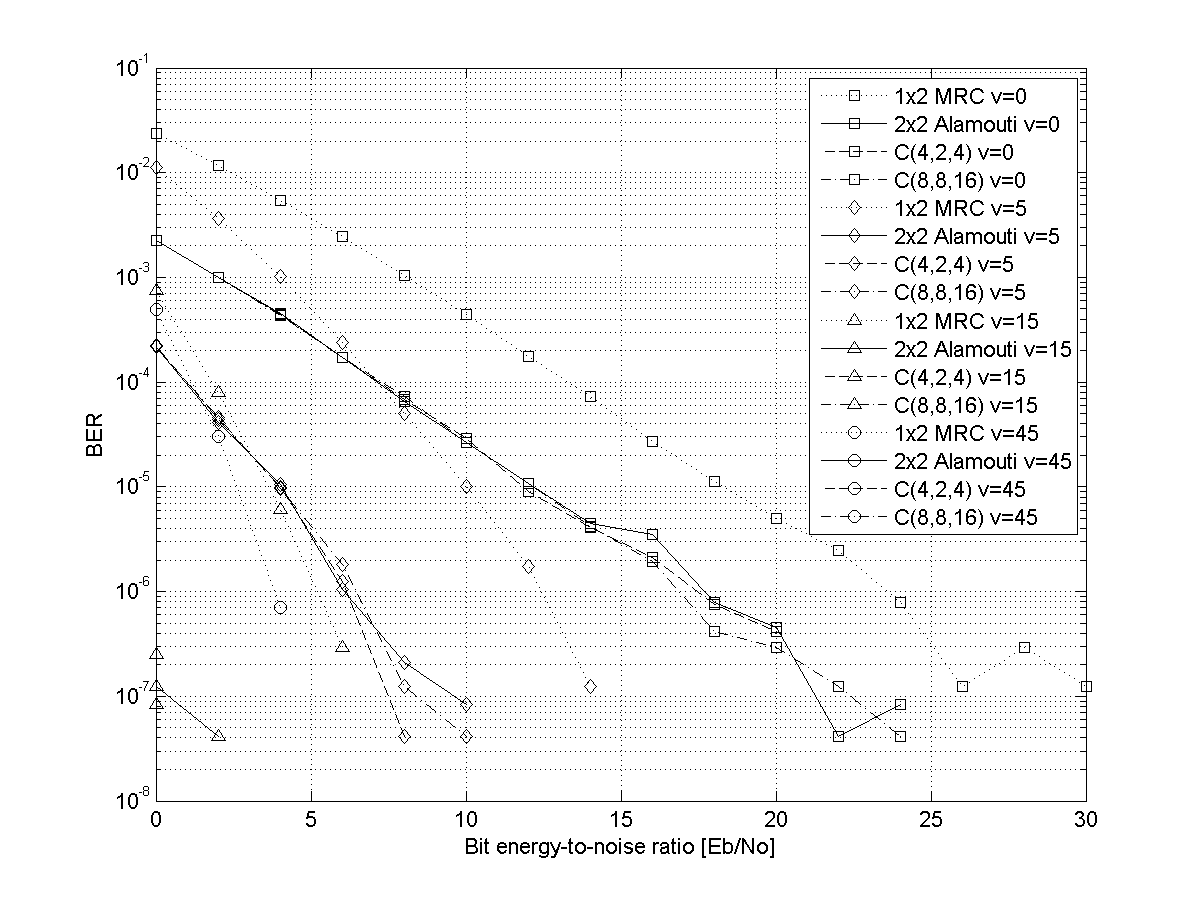
\includegraphics[width=0.8\textwidth]{images/result5.png}
  \caption{Comparison of BER versus $E_b/N_0$ for QPSK, various $N_T$, and moving receiver.}
  \label{fig:result5}
\end{figure}